\chapter{Measurement, Density Matrices, and Entropy}

The two-slit experiment contains the measurement problem in its smallest useful form. When two alternatives remain coherent, their amplitudes interfere. When another system acquires a record of the alternative taken, the object and the recorder become entangled, and the interference changes. We shall make that mechanism exact before introducing the trace, the density matrix, and entropy---the language needed to quantify entanglement.

\section{Rebuilding the Two-Slit Experiment}

Consider a discrete model with a source at site \(0\), two openings \(A\) and \(B\), and a screen whose possible arrival sites are represented by orthonormal states \(\{|m\rangle\}\). The particle may be an electron, a photon, or any other quantum object. We call it an electron, and we ignore its own spin so that position is the only degree of freedom under discussion. The rest of the barrier is closed: an electron reaching any site other than \(A\) or \(B\) is reflected.

The structural principle is linearity. If two states evolve as
\begin{equation}
|A\rangle\longrightarrow |A'\rangle,
\qquad
|B\rangle\longrightarrow |B'\rangle,
\end{equation}
then every superposition evolves with the same coefficients:
\begin{equation}
\alpha|A\rangle+\beta|B\rangle
\longrightarrow
\alpha|A'\rangle+\beta|B'\rangle.
\end{equation}

In a symmetric arrangement the source feeds the two openings with equal amplitude. Suppressing the common normalization, as on the board,
\begin{equation}
|0\rangle\longrightarrow |A\rangle+|B\rangle.
\end{equation}
The normalized state would be \((|A\rangle+|B\rangle)/\sqrt{2}\); the omitted factor plays no role in the interference argument.

Now study each route separately. Propagation from the openings to the screen has the form
\begin{align}
|A\rangle &\longrightarrow \sum_m \psi_m|m\rangle, \\
|B\rangle &\longrightarrow \sum_m \phi_m|m\rangle.
\end{align}
The complex number \(\psi_m\) is the amplitude to arrive at screen site \(m\) after starting at \(A\), and \(\phi_m\) is the corresponding amplitude after starting at \(B\).

\begin{figure}[htbp]
\centering

\includegraphics[width=0.68\textwidth]{lecture_07_figure_02.png}
\caption{The separate \(A\)- and \(B\)-route expansions in the screen basis.}
\lectureframe{00:05:39}
\end{figure}

If \(B\) is closed, the probability at \(m\) is
\begin{equation}
P_A(m)=|\psi_m|^2.
\end{equation}
If \(A\) is closed,
\begin{equation}
P_B(m)=|\phi_m|^2.
\end{equation}
Classical probability would suggest adding these two answers when both openings are available. Quantum mechanics instead adds the amplitudes first:
\begin{equation}
|A\rangle+|B\rangle
\longrightarrow
\sum_m(\psi_m+\phi_m)|m\rangle.
\end{equation}
At a fixed screen site,
\begin{align}
P(m)
&=|\psi_m+\phi_m|^2 \\
&=|\psi_m|^2+|\phi_m|^2
  +\psi_m^*\phi_m+\phi_m^*\psi_m.
\end{align}

\begin{figure}[htbp]
\centering

\includegraphics[width=0.70\textwidth]{lecture_07_figure_03.png}
\caption{The four-term screen probability. The last two terms are the interference terms.}
\lectureframe{00:09:21}
\end{figure}

At a symmetry point, \(\psi_m=\phi_m\), and the two alternatives reinforce one another. At a point where their phases differ by \(\pi\), \(\psi_m=-\phi_m\), the probability vanishes. Either route alone can reach that point, yet opening both routes can prevent the electron from arriving there. The question is now unavoidable: what changes when something records which opening was used?

\section{A Detector Becomes Entangled}

Introduce an auxiliary two-state system with states \(|u\rangle\) and \(|d\rangle\). It is not the electron's spin in this model; it is a minimal external apparatus. Initially the detector is untriggered:
\begin{equation}
|0,d\rangle.
\end{equation}
Arrange the interaction so that passage through \(A\) flips the detector, whereas passage through \(B\) leaves it unchanged:
\begin{equation}
|0,d\rangle
\longrightarrow
|A,u\rangle+|B,d\rangle.
\end{equation}
After the electron leaves the openings, it no longer interacts with the auxiliary spin. The two branches therefore propagate as
\begin{align}
|A,u\rangle &\longrightarrow \sum_m\psi_m|m,u\rangle, \\
|B,d\rangle &\longrightarrow \sum_m\phi_m|m,d\rangle,
\end{align}
and the final state is
\begin{equation}
|\Psi\rangle
=\sum_m\left(\psi_m|m,u\rangle+\phi_m|m,d\rangle\right).
\end{equation}
The route and the detector record are now entangled. Reading the detector would reveal which opening was used.

\begin{classroomqa}
\lecturetimestamp{00:13:24}
\audiencequestion{Has the wave packet already collapsed when the spin flips?}
\lecturerresponse{For the electron alone, one may use collapse language: the path alternatives no longer interfere. For the complete electron--detector system, however, neither branch has been discarded. The state is still \(|A,u\rangle+|B,d\rangle\). Including the apparatus replaces the statement \emph{the electron collapsed} by the precise statement that system--apparatus entanglement was established.}
\end{classroomqa}

The auxiliary spin is only a convenient pointer. A fired or unfired device, an emitted or absent photon, or any other pair of distinguishable records can play the same role.

\begin{classroomqa}
\lecturetimestamp{00:15:17}
\audiencequestion{Does passing through the metal plate itself always leave a path record?}
\lecturerresponse{Not necessarily. What matters is whether the interaction leaves the plate in distinguishable final states. If the plate has an excitation gap and the electron lacks enough energy to excite it, no lasting internal mark need be left. Mere interaction is not enough; the two alternatives must become correlated with distinguishable records.}
\end{classroomqa}

\begin{classroomqa}
\lecturetimestamp{00:16:29}
\audiencequestion{Could the plate's recoil reveal whether the electron passed through the upper or lower opening?}
\lecturerresponse{Only if the opposite momentum kicks produce sufficiently distinguishable plate states. A well-localized plate already has a broad momentum wave function. Small upward and downward shifts can overlap almost completely, so the recoil states are not orthogonal and do not provide an unambiguous route record. This is where the uncertainty principle protects interference.}
\end{classroomqa}

A partial record is possible. If the detector is kicked only slightly, the two final record states need not be orthogonal. Interference is then reduced rather than eliminated. For the formal calculation we first take the limiting case of a complete measurement:
\begin{equation}
\langle u|d\rangle=0.
\end{equation}

\section{The Projector Calculation}

We now calculate the probability that the electron arrives at a fixed screen site \(m\), without asking for the detector outcome. In the combined Hilbert space, the property \emph{electron at \(m\)} is a two-dimensional subspace spanned by
\begin{equation}
|m,u\rangle,\qquad |m,d\rangle.
\end{equation}
The corresponding projector is
\begin{equation}
\Pi_m
=|m,u\rangle\langle m,u|
 +|m,d\rangle\langle m,d|.
\end{equation}

\begin{figure}[htbp]
\centering

\includegraphics[width=0.66\textwidth]{lecture_07_figure_04.png}
\caption{The projector onto a fixed screen position, summed over the two orthogonal detector records.}
\lectureframe{00:22:04}
\end{figure}

The probability postulate gives
\begin{equation}
P(m)=\langle\Psi|\Pi_m|\Psi\rangle.
\end{equation}
Writing out the sums,
\begin{align}
P(m)
&=
\sum_{n,n'}
\left(\psi_n^*\langle n,u|+\phi_n^*\langle n,d|\right)
\notag\\
&\quad\times\Pi_m
\notag\\
&\quad\times
\left(\psi_{n'}|n',u\rangle+\phi_{n'}|n',d\rangle\right).
\end{align}
The position inner products require \(n=m=n'\). The detector inner products then decide which terms remain:
\begin{align}
\langle u|u\rangle&=1,
&
\langle d|d\rangle&=1,
&
\langle u|d\rangle&=\langle d|u\rangle=0.
\end{align}
Consequently,
\begin{equation}
P(m)=|\psi_m|^2+|\phi_m|^2.
\end{equation}

The cross terms have not been removed by decree. They vanish because the two route amplitudes now multiply orthogonal vectors of the enlarged state space. To interfere, alternatives must agree not only at the screen endpoint but in every degree of freedom that carries a record.

\section{What Counts as a Measurement?}

The clean spin model supplies a general rule: measurement occurs when an interaction establishes a correlation between alternatives of the system and distinguishable states of an apparatus. The following variations test that rule.

\begin{classroomqa}
\lecturetimestamp{00:26:53}
\audiencequestion{What if the spin is placed symmetrically and flips for passage through either opening?}
\lecturerresponse{Then both branches carry the same record, \(|A,u\rangle+|B,u\rangle=(|A\rangle+|B\rangle)\otimes|u\rangle\). The detector state factors out and reveals no route information, so the interference pattern remains.}
\end{classroomqa}

\begin{figure}[htbp]
\centering

\includegraphics[width=0.68\textwidth]{lecture_07_figure_05.png}
\caption{The board variation in which a symmetrically placed detector responds identically to both routes.}
\lectureframe{00:27:14}
\end{figure}

\begin{figure}[htbp]
\centering
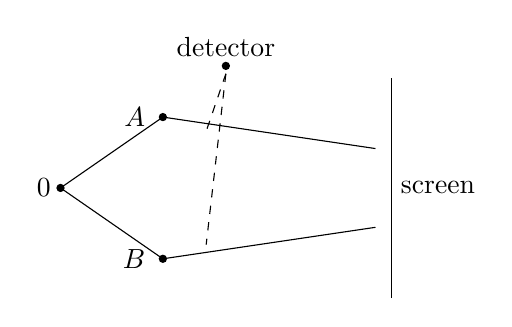
\begin{tikzpicture}[scale=1.0]
\fill (-2,0) circle (1.5pt);
\node[left] at (-2,0) {$0$};
\fill (-0.7,0.9) circle (1.5pt);
\node[left] at (-0.8,0.9) {$A$};
\fill (-0.7,-0.9) circle (1.5pt);
\node[left] at (-0.8,-0.9) {$B$};
\draw (-2,0) -- (-0.7,0.9);
\draw (-2,0) -- (-0.7,-0.9);
\draw (-0.7,0.9) -- (2.0,0.5);
\draw (-0.7,-0.9) -- (2.0,-0.5);
\draw (2.2,-1.4) -- (2.2,1.4);
\node[right] at (2.2,0) {screen};
\fill (0.1,1.55) circle (1.5pt);
\node[above] at (0.1,1.55) {detector};
\draw[dashed] (0.1,1.45) -- (-0.15,0.72);
\draw[dashed] (0.1,1.45) -- (-0.15,-0.72);
\end{tikzpicture}
\caption{A clean reconstruction of the symmetric detector placement: both routes produce the same detector state.}
\end{figure}

\begin{classroomqa}
\lecturetimestamp{00:27:55}
\audiencequestion{Must someone actually read the auxiliary spin before interference disappears?}
\lecturerresponse{No. The electron has already correlated its route with the spin. One may reset the detector, repeat the experiment one electron at a time, and inspect only the distribution of screen hits. The fringes are absent even if nobody reads the spin; the physical record, not human awareness of it, matters.}
\end{classroomqa}

\begin{classroomqa}
\lecturetimestamp{00:29:36}
\audiencequestion{Would a sufficiently light recoiling plate destroy interference?}
\lecturerresponse{Yes, if the recoil shifts the plate into orthogonal momentum states for the two routes. If the shifted wave packets still overlap, the destruction is only partial. Mass by itself is not the criterion; distinguishability of the final plate states is.}
\end{classroomqa}

Radiation provides another imperfect recorder. An accelerated charged particle may emit a photon. Radiation emitted near \(A\) need not be the same state as radiation emitted near \(B\), so the electromagnetic field can retain route information. For a slowly deflected electron the emission probability may be small; the lecture uses an illustrative estimate of roughly one event in a hundred. Stronger acceleration makes radiation and therefore loss of contrast more likely. The important point is qualitative: even an unobserved photon can carry away coherence.

\begin{classroomqa}
\lecturetimestamp{00:32:00}
\audiencequestion{How does one infer the interference probability in a real experiment with imperfect contrast?}
\lecturerresponse{One repeats the experiment many times and estimates the screen distribution from relative frequencies. Finite samples and environmental records leave residual counts in nominally dark regions. The inferred probability distribution improves with the number of trials, while decohering processes reduce the physical fringe contrast.}
\end{classroomqa}

\begin{classroomqa}
\lecturetimestamp{00:33:13}
\audiencequestion{Does any possibility of determining the route destroy all interference?}
\lecturerresponse{Complete distinguishability destroys it completely. Partial information produces partial loss. A detector that rotates only slightly leaves two nonorthogonal record states, so one route becomes more likely than the other when the detector is read, but not certain; correspondingly, the fringes are blurred rather than erased.}
\end{classroomqa}

Let \(|E_A\rangle\) and \(|E_B\rangle\) denote arbitrary record states. The combined state at the screen can be written
\begin{equation}
|\Psi\rangle
=\sum_m\left(
\psi_m|m\rangle|E_A\rangle
+\phi_m|m\rangle|E_B\rangle
\right).
\end{equation}
Ignoring the record system gives
\begin{align}
P(m)
&=|\psi_m|^2+|\phi_m|^2 \\
&\quad
+\psi_m^*\phi_m\langle E_A|E_B\rangle
+\phi_m^*\psi_m\langle E_B|E_A\rangle.
\end{align}
Thus the overlap \(\langle E_A|E_B\rangle\) is the coherence factor. Identical records preserve full interference; orthogonal records remove it; intermediate overlap gives intermediate visibility.

\begin{classroomqa}
\lecturetimestamp{00:34:12}
\audiencequestion{If photons are emitted only occasionally, what happens when one keeps only the photon-emission events?}
\lecturerresponse{That selected subensemble generally has poorer interference because a photon carries route information. The loss need not be complete: photon wave packets emitted at the two openings may themselves overlap, so even the radiative records may fail to be perfectly orthogonal.}
\end{classroomqa}

Environmental bombardment scales this mechanism up. Air molecules, ambient photons, and surrounding matter continuously acquire records of macroscopic positions. A person or the Moon does not remain visibly spread into a coherent position superposition: mass slows free spreading, and continual environmental entanglement suppresses observable interference between macroscopically separated alternatives.

\begin{classroomqa}
\lecturetimestamp{00:36:02}
\audiencequestion{Is this already a theory of measurement, rather than merely another use of the phrase \emph{wave-packet collapse}?}
\lecturerresponse{It is the mechanism in a deliberately exact example. In an electron-only description, collapse means discarding the off-diagonal \(\psi^*\phi\) terms. In the composite description no ad hoc deletion is needed: entanglement with orthogonal apparatus states makes those terms unavailable to measurements on the electron alone. More complicated examples should be traced back to this structure.}
\end{classroomqa}

\begin{classroomqa}
\lecturetimestamp{00:38:04}
\audiencequestion{Would a gravitational field that bends the route naturally change the radiation argument or the interference rule?}
\lecturerresponse{The detailed radiation may change, and quantum mechanics does not assign a single sharp trajectory before a path measurement. The general conclusion does not change: only a degree of freedom that retains distinguishable route information suppresses interference. A concrete apparatus must be specified before a more detailed answer is meaningful.}
\end{classroomqa}

\begin{classroomqa}
\lecturetimestamp{00:39:44}
\audiencequestion{Is this interference different from the interference of classical electromagnetic waves?}
\lecturerresponse{For many photons, the observed pattern agrees with ordinary wave interference of the electromagnetic field. The single-particle experiment shows the deeper quantum statement: photons and electrons arrive as individual events, while their quantum amplitudes interfere. For electrons the relevant wave is the electron wave function, not an electromagnetic wave.}
\end{classroomqa}

\begin{classroomqa}
\lecturetimestamp{00:40:45}
\audiencequestion{What happens to portions of the initial wave aimed between \(A\) and \(B\)?}
\lecturerresponse{In this deliberately discrete model the rest of the barrier is blocked. Those portions are reflected and do not contribute to the transmitted screen amplitude. The model isolates the two transmitted alternatives without claiming that a real beam has only two momentum components.}
\end{classroomqa}

\section{The Cat, the Screen, and the Movable Cut}

The same mathematics applies to Schr\"odinger's cat. Let the gun have states \(|U\rangle\) and \(|F\rangle\) for unfired and fired, and let the cat have states \(|L\rangle\) and \(|D\rangle\) for live and dead. Starting from a live cat and an unfired gun, the interaction may produce
\begin{equation}
|\Psi_{\mathrm{cat}}\rangle
=\alpha|L,U\rangle+\beta|D,F\rangle.
\end{equation}
The cat alone is not in the coherent state \(\alpha|L\rangle+\beta|D\rangle\). It is entangled with a gun that has recorded the alternative. Looking at the gun can reveal the cat's branch, and the orthogonal gun records remove ordinary live--dead interference in the cat subsystem.

\begin{classroomqa}
\lecturetimestamp{00:41:18}
\audiencequestion{Is the cat itself in a superposition of alive and dead?}
\lecturerresponse{Not in the simple isolated sense. The composite cat--gun system is in a superposition of correlated alternatives, live with unfired and dead with fired. The cat subsystem is entangled with a record-bearing gun, exactly as the electron route is entangled with the auxiliary spin.}
\end{classroomqa}

The final screen also has to be treated as an apparatus. An electron arriving at \(m\) may blacken a photographic grain, make a scintillator emit a photon, or flip one detector in a row of local two-state devices. The mark becomes correlated with the arrival position.

\begin{classroomqa}
\lecturetimestamp{00:43:38}
\audiencequestion{Why may we speak of probabilities at the final screen rather than carry only state vectors forever?}
\lecturerresponse{The probability postulate assigns \(\langle\Pi_m\rangle\) to the property \emph{arrival at \(m\)}. To complete the physical experiment, the screen then leaves a position record. The projector gives the probability; blackening, scintillation, or a local detector flip realizes the measurement whose statistics are being collected.}
\end{classroomqa}

\begin{classroomqa}
\lecturetimestamp{00:45:00}
\audiencequestion{Why discuss a screen measurement but not a probability for passage through \(A\) or \(B\)?}
\lecturerresponse{One may assign and test path probabilities only by installing a path recorder. Without such a record the alternatives remain coherent and must be added as amplitudes. At the screen, a position-sensitive apparatus is assumed. The difference is not a privileged time but whether a corresponding measurement interaction has been arranged.}
\end{classroomqa}

The boundary between system and apparatus can be moved. Include an observer with record states \(|O_u\rangle\) and \(|O_d\rangle\); then
\begin{equation}
|A,u\rangle+|B,d\rangle
\longrightarrow
|A,u,O_u\rangle+|B,d,O_d\rangle.
\end{equation}
Another observer may in turn become correlated with the first. Smoke in the cat's box, the gun, the cat, Schr\"odinger, and Wigner can all be included in one longer entanglement chain. Wherever the cut is drawn, the correlations must remain consistent: if Wigner later asks Schr\"odinger what he saw, their records agree.

\begin{classroomqa}
\lecturetimestamp{00:47:24}
\audiencequestion{Where exactly should the system end and the measuring observer begin?}
\lecturerresponse{Quantum mechanics does not select a unique convenient cut. One may collapse the electron-only description, include the detector and collapse a larger description, or include an observer and enlarge the entangled state again. The physical requirement is consistency of all accessible probabilities and records, not a unique bookkeeping boundary.}
\end{classroomqa}

\begin{classroomqa}
\lecturetimestamp{00:49:47}
\audiencequestion{Does the uncertainty principle enter because measuring the path disturbs the event?}
\lecturerresponse{Yes. The recoil example makes the connection explicit: localization of the plate produces momentum uncertainty, which can prevent small path-dependent kicks from becoming distinguishable. More generally, a quantum measurement is not complete until system--apparatus entanglement has changed the state, and that change can alter later interference.}
\end{classroomqa}

This marks a sharp contrast with the classical ideal. Classically one imagines making a measurement arbitrarily gentle, extracting information with negligible disturbance. Here extracting path information requires establishing a correlation with an apparatus. That is a genuine change of the joint state, and it changes the answer to a later interference experiment.

\begin{classroomqa}
\lecturetimestamp{00:52:06}
\audiencequestion{What happens if the separation between \(A\) and \(B\) becomes very large?}
\lecturerresponse{There is no universal new rule. In this source-and-barrier geometry the amplitudes to reach very distant openings may simply become small, so most particles hit the blocked region. Apart from such apparatus-dependent changes in \(\psi_m\) and \(\phi_m\), separation alone does not decide whether coherence survives.}
\end{classroomqa}

\begin{classroomqa}
\lecturetimestamp{00:53:04}
\audiencequestion{Is the linearity of quantum evolution fundamentally exact, and why does nature use it?}
\lecturerresponse{Linearity is an empirical foundation of quantum mechanics. Small nonlinear modifications are notoriously difficult to make logically coherent and tend to spoil the structure. The deeper reason that physical propositions follow the logic of subspaces rather than classical sets is not supplied here; the lecture treats it as a fact of nature.}
\end{classroomqa}

\begin{classroomqa}
\lecturetimestamp{00:54:53}
\audiencequestion{Could a later observation reveal the earlier path and thereby change whether interference occurred?}
\lecturerresponse{If a later observation can reveal the path, some physical degree of freedom must have preserved a path-dependent record. That record already affects coherence; nobody has to read it. Causality must still be respected, and an abstract delayed-choice claim cannot be settled without specifying the complete spacetime arrangement and apparatus.}
\end{classroomqa}

\begin{classroomqa}
\lecturetimestamp{00:56:47}
\audiencequestion{What if a bubble chamber is placed immediately after the openings?}
\lecturerresponse{A track that distinguishes the two emerging routes is an unambiguous mark, so it destroys their interference. A thin path-recording layer is enough. If a downstream device does not retain enough information to infer the earlier opening, then it does not automatically serve as a which-path detector.}
\end{classroomqa}

\begin{classroomqa}
\lecturetimestamp{00:59:29}
\audiencequestion{If the world is already highly entangled, how can an interference experiment ever begin with disentangled systems?}
\lecturerresponse{The preparation must isolate, reset, or condition the relevant degrees of freedom well enough that the alternatives start with the same environmental record. A prior bubble-chamber track cannot simply be ignored if it remains correlated with the path. Interference requires a product-like initial relation between the controlled system and the relevant recorder.}
\end{classroomqa}

\begin{classroomqa}
\lecturetimestamp{01:01:04}
\audiencequestion{Where does practical disentanglement come from after a measurement?}
\lecturerresponse{Condition on a definite observed outcome. If the spin is found up, the observer retains the branch \(|A,u\rangle\) and discards the alternative from the working description. That conditional product state can be used as a new starting point. The full observer-inclusive state may remain entangled, but relative to the recorded outcome the selected preparation is definite.}
\end{classroomqa}

This nested hierarchy does not resolve every interpretive question, but it makes the operational consistency visible. System, detector, observer, and observer of observer may all be included. No matter where the description is cut, correctly correlated records do not later contradict one another.

\section{From Entanglement to Entropy}

The discussion has gone farther into measurement than planned, but it has exposed the next question: how can the degree of entanglement be measured? Two spins in the product state
\begin{equation}
|u\rangle\otimes|u\rangle
\end{equation}
are not entangled. Each subsystem has its own definite state, and observing one supplies no new information about the other. Entangled states do not factor this way. A standard quantitative diagnostic will be entanglement entropy, but we first need the ordinary notion of entropy and then its quantum form.

\section{Classical Entropy as Missing Information}

Begin with a classical system having a finite set of \(N\) possible states. Entropy here is a property of the system together with our knowledge of it. Suppose all we know is that the system occupies one of \(n\) equally probable states. Then
\begin{equation}
S=\log n.
\end{equation}
If \(n=1\), the state is known and \(S=0\). If \(n=N\), nothing is known beyond the state space itself and the entropy is maximal, \(S_{\max}=\log N\).

The logarithm counts independent yes--no choices additively. For \(M\) classical spins there are \(2^M\) configurations, so
\begin{equation}
\log(2^M)=M\log 2.
\end{equation}
Up to the choice of logarithm base, entropy therefore counts the amount of binary information missing from the description.

For a general probability distribution \(p_i\), the appropriate definition is
\begin{equation}
S=-\sum_i p_i\log p_i.
\end{equation}

\begin{classroomqa}
\lecturetimestamp{01:14:17}
\audiencequestion{Why is there a minus sign in the entropy formula?}
\lecturerresponse{Every nonzero probability satisfies \(0<p_i\leq 1\), so \(\log p_i\leq 0\). The minus sign makes entropy nonnegative. At \(p_i=0\), the contribution is defined by the limit \(p_i\log p_i\to0\).}
\end{classroomqa}

For the equal-probability distribution
\begin{equation}
p_i=
\begin{cases}
1/n, & i\in\mathcal N,\\
0, & i\notin\mathcal N,
\end{cases}
\qquad |\mathcal N|=n,
\end{equation}
the general formula becomes
\begin{align}
S
&=-n\left(\frac1n\right)\log\left(\frac1n\right)\\
&=\log n.
\end{align}
It therefore reproduces the elementary counting definition. A distribution concentrated with certainty on one state has \(S=0\).

\begin{figure}[htbp]
\centering

\includegraphics[width=0.66\textwidth]{lecture_07_figure_07.png}
\caption{The board collects \(S=\log n\), the Shannon formula, and the equal-probability check.}
\lectureframe{01:16:08}
\end{figure}

\begin{classroomqa}
\lecturetimestamp{01:17:35}
\audiencequestion{What is the largest entropy a system with \(N\) states can have, and what is known in that case?}
\lecturerresponse{The maximum is \(\log N\), attained by the uniform distribution \(p_i=1/N\). One still knows what the system is and therefore knows its state space; what is unknown is which of those \(N\) states it occupies.}
\end{classroomqa}

The difference
\begin{equation}
I=S_{\max}-S
\end{equation}
is the available information in this counting sense. Entropy and information are opposite sides of the same bookkeeping: entropy records information that could distinguish the state but is not available to us.

\section{Trace: the Quantum Replacement for a Sum}

For an operator \(M\) and any complete orthonormal basis \(\{|i\rangle\}\), define
\begin{equation}
\operatorname{Tr}M
=\sum_i\langle i|M|i\rangle.
\end{equation}

\begin{figure}[htbp]
\centering

\includegraphics[width=0.68\textwidth]{lecture_07_figure_08.png}
\caption{The trace written as the sum of diagonal matrix elements.}
\lectureframe{01:21:20}
\end{figure}

Although the definition is written using a basis, the result is basis independent. For a Hermitian operator one may choose an eigenbasis, in which
\begin{equation}
\operatorname{Tr}M=\sum_i\lambda_i.
\end{equation}
The eigenvalues, and hence their sum, do not depend on the coordinates used to represent the operator.

\begin{classroomqa}
\lecturetimestamp{01:23:04}
\audiencequestion{Does putting a matrix in diagonal form imply that it has an inverse?}
\lecturerresponse{No. Diagonal form displays the eigenvalues; invertibility is a separate condition. A diagonal matrix is invertible precisely when none of its diagonal eigenvalues is zero. Hermitian matrices are diagonalizable even when some eigenvalues vanish.}
\end{classroomqa}

After the break, return briefly to classical probability. A classical observable is a function \(f_i\) of the configuration, and its average is
\begin{equation}
\langle f\rangle_{\mathrm{cl}}=\sum_i p_i f_i.
\end{equation}
In the quantum formulas, the trace will replace the sum over alternatives, an operator will replace the classical function, and a density matrix will replace the probability distribution.

\section{Statistical Mixtures and the Density Matrix}

Suppose someone prepares a system in one state of an orthonormal basis but does not tell us which state was chosen. They provide only preparation probabilities---for example, a spin is prepared up with probability \(3/4\) and down with probability \(1/4\). This is not the coherent superposition
\begin{equation}
\sqrt{\frac34}|u\rangle+\sqrt{\frac14}|d\rangle,
\end{equation}
because no relative phase has been prepared. It is a statistical mixture of definite states. Quantum probabilities remain even when a pure state is known; here there is an additional uncertainty about which pure state was prepared.

\begin{figure}[htbp]
\centering

\includegraphics[width=0.66\textwidth]{lecture_07_figure_06.png}
\caption{The conceptual transition from a specified ket to an ensemble description.}
\lectureframe{01:29:43}
\end{figure}

If state \(|i\rangle\) is prepared with probability \(\rho_i\), the density operator is
\begin{equation}
\rho=\sum_i\rho_i|i\rangle\langle i|.
\end{equation}
In the preparation basis,
\begin{equation}
\rho=
\begin{pmatrix}
\rho_1&0&0&\cdots\\
0&\rho_2&0&\cdots\\
0&0&\rho_3&\cdots\\
\vdots&\vdots&\vdots&\ddots
\end{pmatrix}.
\end{equation}

\begin{figure}[htbp]
\centering

\includegraphics[width=0.68\textwidth]{lecture_07_figure_09.png}
\caption{The diagonal density matrix and its normalization condition.}
\lectureframe{01:32:12}
\end{figure}

Its eigenvalues are real and nonnegative, and normalization of probabilities becomes
\begin{equation}
\operatorname{Tr}\rho=\sum_i\rho_i=1.
\end{equation}

Let \(F\) be a Hermitian observable. The ensemble expectation value is
\begin{equation}
\langle F\rangle=\operatorname{Tr}(F\rho).
\end{equation}

\begin{figure}[htbp]
\centering

\includegraphics[width=0.68\textwidth]{lecture_07_figure_10.png}
\caption{The trace expectation value \(\langle F\rangle=\operatorname{Tr}(F\rho)\).}
\lectureframe{01:35:05}
\end{figure}

To recover the ordinary weighted average, evaluate the trace in the basis where \(\rho\) is diagonal and insert the resolution of identity:
\begin{align}
\operatorname{Tr}(F\rho)
&=\sum_i\langle i|F\rho|i\rangle\\
&=\sum_{i,j}\langle i|F|j\rangle
               \langle j|\rho|i\rangle\\
&=\sum_i\rho_i\langle i|F|i\rangle.
\end{align}
Thus each pure-state expectation value is weighted by the probability that the corresponding state was prepared.

The trace has the cyclic property
\begin{equation}
\operatorname{Tr}(AB)=\operatorname{Tr}(BA),
\end{equation}
even if \(A\) and \(B\) do not commute. Hence \(\operatorname{Tr}(F\rho)=\operatorname{Tr}(\rho F)\).

\section{Quantum Entropy and the Deferred Payoff}

The entropy of a density matrix is
\begin{equation}
S(\rho)=-\operatorname{Tr}(\rho\log\rho).
\end{equation}
For a Hermitian positive operator, functions such as \(\log\rho\) are defined through its eigenvalues. If
\begin{equation}
\rho=\sum_i\rho_i|i\rangle\langle i|,
\end{equation}
then
\begin{equation}
\log\rho=\sum_{\rho_i>0}(\log\rho_i)|i\rangle\langle i|,
\end{equation}
and therefore
\begin{equation}
S(\rho)=-\sum_i\rho_i\log\rho_i.
\end{equation}

\begin{figure}[htbp]
\centering

\includegraphics[width=0.68\textwidth]{lecture_07_figure_11.png}
\caption{The classical entropy formula recast as \(S=-\operatorname{Tr}(\rho\log\rho)\).}
\lectureframe{01:41:25}
\end{figure}

A known pure state has density operator
\begin{equation}
\rho_\psi=|\psi\rangle\langle\psi|,
\end{equation}
with eigenvalues \(1,0,\ldots\), so \(S(\rho_\psi)=0\). This does not mean that every measurement on \(|\psi\rangle\) has a certain outcome. It means there is no additional statistical ignorance about the prepared state. At the opposite extreme,
\begin{equation}
\rho=\frac{I}{d}
\qquad\Longrightarrow\qquad
S(\rho)=\log d,
\end{equation}
where \(d=\dim\mathcal H\). The maximally mixed state assigns equal weight to every orthogonal direction.

The connection to entanglement is now close but not yet worked out. Suppose a composite system \(AB\) is in a joint state and all experiments are confined to \(A\). There must be an object that reproduces every expectation value obtainable on \(A\) while \(B\) is ignored. That object is a density matrix for \(A\). If the joint state factorizes, the density matrix of \(A\) is pure and has zero entropy. If \(A\) and \(B\) are entangled, the density matrix of \(A\) is generally mixed and has nonzero entropy. Constructing that reduced density matrix and evaluating its entropy is the task reserved for the next lecture.
